\documentclass{article}
\usepackage{graphicx}
\usepackage[utf8]{inputenc}
\usepackage{listings}
\usepackage{color}
\usepackage{xcolor}
\usepackage{textcomp}
\usepackage{amsmath}
\usepackage{mathabx}

\definecolor{solarized@base03}{HTML}{002B36}
\definecolor{solarized@base02}{HTML}{073642}
\definecolor{solarized@base01}{HTML}{586e75}
\definecolor{solarized@base00}{HTML}{657b83}
\definecolor{solarized@base0}{HTML}{839496}
\definecolor{solarized@base1}{HTML}{93a1a1}
\definecolor{solarized@base2}{HTML}{EEE8D5}
\definecolor{solarized@base3}{HTML}{FDF6E3}
\definecolor{solarized@yellow}{HTML}{B58900}
\definecolor{solarized@orange}{HTML}{CB4B16}
\definecolor{solarized@red}{HTML}{DC322F}
\definecolor{solarized@magenta}{HTML}{D33682}
\definecolor{solarized@violet}{HTML}{6C71C4}
\definecolor{solarized@blue}{HTML}{268BD2}
\definecolor{solarized@cyan}{HTML}{2AA198}
\definecolor{solarized@green}{HTML}{859900}

\lstset{
  language=Python,
  upquote=true,
  columns=fixed,
  tabsize=2,
  extendedchars=true,
  breaklines=true,
  frame=single,
  numbers=left,
  numbersep=5pt,
  rulesepcolor=\color{solarized@base03},
  numberstyle=\tiny\color{solarized@base01},
  basicstyle=\footnotesize\ttfamily,
  keywordstyle=\color{solarized@green},
  stringstyle=\color{solarized@cyan}\ttfamily,
  identifierstyle=\color{solarized@blue},
  commentstyle=\color{solarized@base01},
  emphstyle=\color{solarized@red}
}
\begin{document}

\title{Tarea Método de Newton}
\author{Angel Caceres Licona}

\maketitle

\section{Considerar la función $f(x) = x^2-4\cos(x) , x \in {\rm I\!R}$...}
\section{Graficar en el intervalo $(1,2)$}

Gráfica

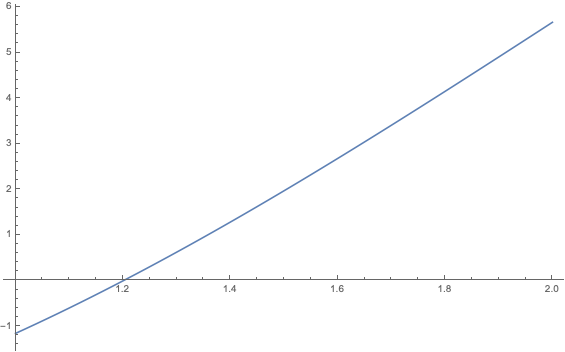
\includegraphics[scale=0.4]{grafica1.png}


\section{Código del programa}

\begin{lstlisting}
    from math import *

    def newtonIterationFunction(x): 
        return x - ((x**2 - 4*cos(x)) / (2*x+4*sin(x)))
     
    
    def function(x): 
        return x**2 - 4*cos(x)
    
    x = 1
    c = 1
    xold = 0
    fc = 1
    
    for i in range(1000):
        print "Iteraciones: ",str(i),"Valor aproximado: ", str(x), "Intervalo", str(c)
        c = (x - xold)
        fc = function(x)
        xold = x
        x = newtonIterationFunction(x) 
        if (abs(fc) < 0.000000005) :
            break
\end{lstlisting}

\subsection{Usar el método de newton para localizar una aproximacion...}


\begin{center}
    \begin{tabular}{||c c c c||} 
    \hline
    $n$ & $p_{i}$ & $E_i$  & $ f(p_i)$ \\ [0.5ex] 
    \hline
    0 & 1.21640595224 & 1 & -1.16120922347 \\
    \hline
    1 & 1.20159918212 & 0.2164059522393 & 0.0915686905446 \\
    \hline
    2 & 1.20153830038 & -0.0148067701169 & 0.000373428376449 \\
    \hline
    3 & 1.20153829934 & -6.08817408994e-05 &  6.38189479041e-09 \\ [1ex]
    \hline

   \end{tabular}
\end{center}

\subsection{Aplicar el método de bisección, secante y falsa posicion con la misma tolerancia...}
Para biseccion salieron 28 iteraciones.
Para secante salieron 8 iteraciones.
Para secante salieron 7 iteraciones.

\section{Considere la funcion $-8e^{1-x} +\frac{7}{x}$}
\subsection{Grafique en el intervalo $(0,2)$}
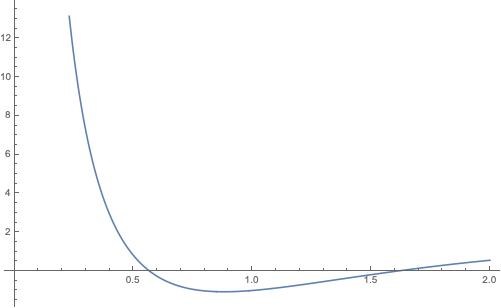
\includegraphics[scale=0.75]{grafica2.png}


\subsection{Con el programa obtengo los siguientes resultados}

\begin{center}
    \begin{tabular}{||c c c c||} 
    \hline
    $n$ & $p_{i}$ & $E_i$  & $ f(p_i)$ \\ [0.5ex] 
    \hline
    0 & 0.55470744502 & 0.5 & 0.810229834399 \\
    \hline
    1 & 0.567540459004 & 0.05470744502 & 0.131690221821 \\
    \hline
    2 & 0.56813355775 & 0.0128330139839 & 0.00557743516944 \\
    \hline
    3 & 0.568134762962 & 0.000593098746384 & 1.1287832983e-05 \\ 
    \hline
    4 & 0.568134762967 & 1.20521197233e-06 &  4.64979166281e-11 \\ [1ex]

   \end{tabular}
\end{center}

\subsection{Compare el resultado con biseccion, secante y punto fijo}
Para biseccion obtuve 28 iteraciones
Para secante obtuve 7 iteraciones
Para falsa posicion obtuve 12 iteraciones

\subsection{Ahora la segunda raiz}

\begin{center}
    \begin{tabular}{||c c c c||} 
    \hline
    $n$ & $p_{i}$ & $E_i$  & $ f(p_i)$ \\ [0.5ex] 
    \hline
    0 & 1.60935506282 & 1.6 & -0.01549308875229 \\
    \hline
    1 & 1.60938106752 & 0.00935506281674 & -4.2828011722e-05 \\
    \hline
    2 & 1.60938106772 & 2.60047028984e-05 & -3.35051986156e-10 \\ [1ex]
    \hline
   \end{tabular}
\end{center}

\subsection{Compare el resultado con biseccion, secante y punto fijo}
Para biseccion obtuve 26 iteraciones
Para secante obtuve 5 iteraciones
Para falsa posicion obtuve 6 iteraciones

\end{document}